\documentclass[a4paper,10pt]{article}
\usepackage[utf8]{inputenc}

\setlength\parindent{0pt}
\usepackage[english]{babel}
\usepackage[dvinames]{xcolor}
\usepackage[compact,small]{titlesec}
\usepackage{booktabs}
\usepackage{multirow}
\usepackage{amsfonts,amsmath,amssymb}
\usepackage{marginnote}
\usepackage[top=1.8cm, bottom=1.8cm, outer=1.8cm, inner=1.8cm, heightrounded, marginparwidth=2.5cm, marginparsep=0.5cm]{geometry}
\usepackage{enumitem}
\setlist{noitemsep,parsep=2pt}
\newcommand{\highlight}[1]{\textcolor{kuleuven}{#1}}
\usepackage{pythonhighlight}
\usepackage{cleveref}
\usepackage{graphicx}
\usepackage{algorithmic}
\usepackage{tabularx}

\newcommand{\nextyear}{\advance\year by 1 \the\year\advance\year by -1}
\newcommand{\thisyear}{\the\year}
\newcommand{\deadlineGroup}{November 27, \thisyear{} at 16:00 CET}
\newcommand{\deadlineCode}{December 18, \thisyear{} at 16:00 CET}
\newcommand{\deadlineReport}{January 4, \nextyear{} at 16:00 CET}

\newcommand{\ReplaceMe}[1]{{\color{blue}#1}}
\newcommand{\RemoveMe}[1]{{\color{purple}#1}}

\setlength{\parskip}{5pt}

%opening
\title{Artificial Neural Networks: Exercise session 2}
\author{Stijn Staring (r0620003)}

\begin{document}
\fontfamily{ppl}
\selectfont{}

\maketitle


\section{Exercises of Section 1: Hopfield Network}
\textbf{Create a Hopfield network with attractors T = [1 1;-1  -1; 1 -1]T and the corresponding number of neurons. You
	can use script rep2 as a basis and modify it to start from some particular points (e.g. of high symmetry) or to generate
	other numbers of points. Start with various initial vectors and note down the obtained attractors after a sufficient number
	of iterations. Are the real attractors the same as those used to create the network? If not, why do we get these unwanted
	attractors? How many iterations does it typically take to reach the attractor? What can you say about the stability of the
	attractors?}\\

In Figure \ref{fig:rep2Attractors} all the found attractors can be seen which are more than the three desired ones that were specified to the Hopfield network. It can thus concluded that the despite the ``newhop'' matlab function tries to design a Hopfield network with the minimum of unspecified target attractors, they often occur. Table \ref{tab:attractors} shows the found attractor points. when designing the energy function for the system that has a corresponding local minima on at the attractor points, it can be that also unwanted attractor points become local minima. When the assumption of no bais term of the model is made, these correspond with the negative of the desired attractors. Also, a mixture of the desired states are possible. The amount of iterations it takes to reach an attractor depends on the start position. All the symmetric starting points of Figure \ref{fig:rep2Attractors} reached an atractor in less then $ 5 $ iterations. However, the amount of iterations can dramatically increase when the starting point is very close to an unstable attractor. For example when the starting point chosen is: $ [-1;-10^{-20}] $ it takes $ 308 $ iteration to reach the stable attractor $ [-1;-1] $. When the system is in a stable attractor and a little noise is added the system will move back to the stable attraction point. An unstable attractor on the other hand will move away when this happens. The stability of the diffent attractor points can be seen in Table \ref{tab:att}.


\begin{figure}[h!]
	\centering
	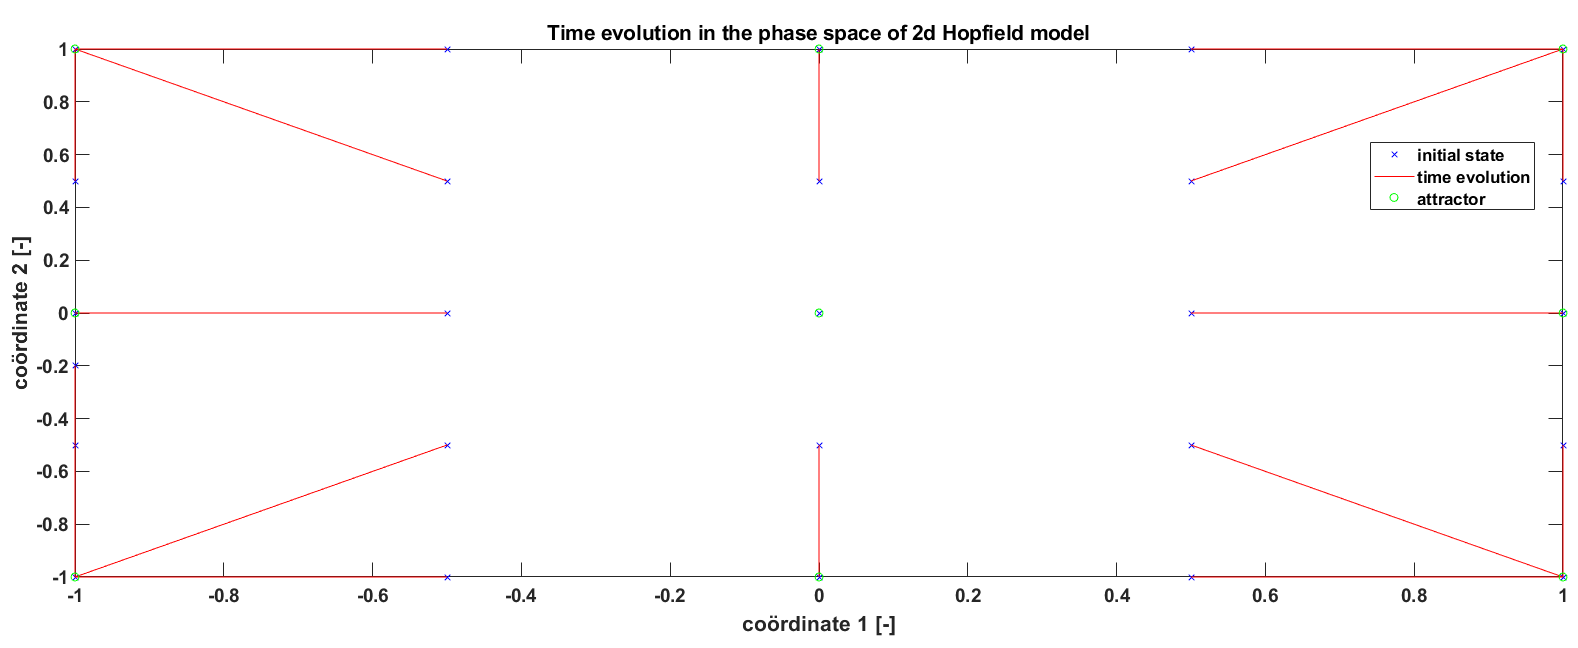
\includegraphics[width=1.\textwidth]{rep2Attractors.png}
	\caption{All the found attractors.}
	\label{fig:rep2Attractors}
\end{figure}


\begin{table}
	\centering
	\begin{tabular}{@{}clr@{}} \toprule
		\textbf{Attractor} & \textbf{Point} & \textbf{Stability}\\\midrule
		Attractor $ 1 $ & $ [1;1] $ & Stable\\
		Attractor $ 2 $ & $ [-1;-1] $ & Stable\\
		Attractor $ 3 $ & $ [1;-1] $ & Stable\\
		Attractor $ 4 $ & $ [-1;1] $ & Stable\\
		Attractor $ 5 $ & $ [0;0] $ & Unstable\\
		Attractor $ 6 $ & $ [0;1] $ & Unstable\\
		Attractor $ 7 $ & $ [0;-1] $ & Unstable\\
		Attractor $ 8 $ & $ [1;0] $ & Unstable\\
		Attractor $ 9 $ & $ [-1;0] $ & Unstable\\\bottomrule
	\end{tabular}
	\caption{Overview of the different attractor points found in a 2D plane.}
	\label{tab:att}
\end{table}

Table \ref{tab:att3} shows an overview of the found attractors in a 3D space. Only the three specified target attractors were found during the experimentation with different starting points. All three are stabel points. 
\begin{table}
	\centering
	\begin{tabular}{@{}clr@{}} \toprule
		\textbf{Attractor} & \textbf{Point} & \textbf{Stability}\\\midrule
		Attractor $ 1 $ & $ [1;1;1] $ & Stable\\
		Attractor $ 2 $ & $ [-1;-1;1] $ & Stable\\
		Attractor $ 3 $ & $ [1;-1;-1] $ & Stable\\\bottomrule
	\end{tabular}
	\caption{Overview of the different attractor points found in a 3D plane.}
	\label{tab:att3}
\end{table}
\newpage
\textbf{The function hopdigit creates a Hopfield network which has as attractors the handwritten digits 0,...,9. Then to test
	the ability of the network to correctly retrieve these patterns some noisy digits are given to the network. Is the Hopfield
	model always able to reconstruct the noisy digits? If not why? What is the influence of the noise on the number of
	iterations?}\\

The noise that is added to the digits is gaussian noise. The noise variable determines the standard deviation of the gaussian that is sampled from to retrieve the noise that should be added. It can be concluded that when the noise is too high, the Hopfield model is not able to reconstruct the correct digits. The reason is because when the noise is too heavy the starting point can become closer to other digits than the original one. Increasing the amount of iterations will not solve this issue. When there is more noise, the system needs more iterations to reach the attractor points.

\section{Exercises of Section 2: Long Short-Term Memory Networks}
















%\cite{fast_alg}
%\cite{inver_over}

\bibliographystyle{abbrv}
%\bibliography{ANN1}

\end{document}
